\documentclass[12pt]{extreport}
\usepackage[a4paper]{geometry}
\usepackage{extsizes}
\usepackage{amsthm}
\usepackage{amsmath}
\usepackage{amssymb}
\usepackage{float}
\usepackage{graphicx}
\newtheorem*{thm}{Theorem}

\begin{document}
\title{MAT 180 Term Paper}
\author{Darya Chumakova and Satoshi Scott Iwako}
\maketitle

\section*{Introduction}
In this paper, we will first present an inductive proof of the Arithmetic-Geometric-Harmonic Mean Inequality and then discuss a recent application to approximating area under a parabola of degree $n \geq 2$ with $f(x) > 0$ for $-1 < x < 1$ and $f(-1) = f(0) = 0$. We chose this topic because we liked the creative ingenuity behind the forward and backward inductive argument. The algebraic proof of the Arithmetic-Geometric Mean Inequality with $n = 2$ was presented to us in Real Analysis, but we have never seen an argument for all $n \in \mathbb{N}$. We have never seen the Harmonic Mean and it's relationship to the other two means prior to this paper, so it was insightful to prove the full inequality and discover it's applications in modern research. 
\section*{History}
The first published record of the arithmetic-geometric mean inequality appeared in a memoir of Lagrange in 1784-1785. However Gauss also independently discovered the arithmetic-geometric mean inequality in 1791 at the age of 14 as evident in his journal and wrote a paper about it at the age of 22 or 23 (the paper was published by E.Schering in 1866 after Gauss's death). Gauss discovered the relationship by looking at the limit of the sequences $\{a_n\}_{n = 0}^{\infty}$ and $\{b_n\}_{n = 0}^{\infty}$ with $a_0 = a, b_0 = b$ and $a_{n+1} = (a_n + b_n)/2, b_{n+1} = (a_nb_n)^{1/2}$ and finding that $\lim_{n\to\infty} a_n = \lim_{n\to\infty} b_n$. Early applications of the inequality include computing elliptical and lemniscatic integrals. In particular, there is a close relationship between the perimeter of an ellipse (or length of an arc of an ellipse) and the arithmetic-geometric mean. One of the main motivations behind this was to approximate elliptical orbits of planets. John Landen applied the arithmetic-geometric mean to Landen's transformation (a mapping of of the parameters of an elliptic integral). Since it's discovery, the arithmetic-geometric mean has also been applied to fields such as approximation of $\pi$ and calculation of elementary functions. In the last decade, the inequality has been used to improve the speed of machine computation. The application we will present in this paper was published by Erdos and Gallai in 1938 in their paper \textit{On Polynomials With Only Real Roots}.

\section*{Geometric-Arithmetic-Harmonic Means}
The geometric mean (GM), arithmetic mean (AM) and harmonic mean (HM) of a set $A = \{a_1, a_2 ... a_n\}$ is defined by:
\begin{align*}
 GM(A) &= \sqrt[n]{a_1a_2 \cdot a_n} \\
 AM(A) &= \frac{a_1 + a_2 + ... + a_n}{n} \\
 HM(a) &= \frac{n}{1/a_1 + 1/a_2 + ... + 1/a_n}
\end{align*} 

In the first part of the paper, we will prove the following inequality relating all three of the above means: 
% Daryas Part
\begin{thm}
For any $n$ positive numbers $a_1, a_2, ... a_n$: 
\begin{align*}
\frac{n}{1/a_1 + 1/a_2 + ... + 1/a_n} \leq \sqrt[n]{a_1 a_2 a_3 ... a_n} \leq \frac{a_1 + a_2 + ... + a_n}{n}
\end{align*}
Where the equality holds iff $a_1 = a_2 = ... = a_n$.
\end{thm}

\begin{proof}
We will first prove:
\begin{align*}
\sqrt[n]{a_1 a_2 a_3 ... a_n} \leq \frac{a_1 + a_2 + ... + a_n}{n}
\end{align*}

\begin{flushleft}
\textit{Forward Induction:} (To show statement holds for $n = 2^k$ where $k = 1, 2, 3...$) \\
\textbf{Base Case:} We wish to show the inequality holds for n = 2 i.e. $$\sqrt{ab} \leq \frac{a+b}{2}$$
Suppose $a$ and $b$ are positive numbers. Then $(a-b)^2 \geq 0$. From here it follows that:
\begin{align*}
(a-b)^2 \geq 0 &\iff a^2 - 2ab + b^2 \geq 0 \\
			   &\iff a^2 + 2ab + b^2 \geq 4ab \\
			   &\iff (a+b)^2 \geq 4ab \\
			   &\iff (a+b) \geq 2\sqrt{ab} \\
			   &\iff \frac{a+b}{2} \geq \sqrt{ab}
\end{align*}
Hence the inequality holds for $n=2$.\\
\textbf{Inductive Step:} Suppose $$\frac{a_1 + a_2 + ... + a_n}{n} \geq \sqrt[n]{a_1 a_2 a_3 ... a_n} \qquad (1)$$ holds for $n = 2^k$. We wish to show the inequality holds for $n = 2^{k+1} = 2 \cdot 2^k = 2n$. Let:
$$a_1 = \frac{b_1 + b_2}{2} \qquad a_2 = \frac{b_3 + b_4}{2} \qquad \ldots \qquad a_n = \frac{b_{2n-1} + b_{2n}}{2}$$
where $b_1, b_2 ... b_{2n}$ are positive numbers. Next, we will substitute the above values into $(1)$. 
\begin{align*}
\frac{ (\frac{b_1 + b_2}{2} + \frac{b_3 + b_4}{2} + \ldots + \frac{b_{2n-1} + b_{2n}}{2}) } {n} \geq \sqrt[n]{(\frac{b_1 + b_2}{2})\cdot(\frac{b_3 + b_4}{2})\cdots (\frac{b_{2n-1} + b_{2n}}{2})} &\iff \\
\frac{b_1 + b_2 + b_3 + b_4 + \ldots + b_{2n-1} + b_{2n}}{2n} \geq \sqrt[n]{(\frac{b_1 + b_2}{2}) \cdot (\frac{b_3 + b_4}{2}) \cdots (\frac{b_{2n-1} + b_{2n}}{2})}
\end{align*}
Next we apply the $n=2$ inequality to each of the terms on the right hand side of the inequality to get the following:
\begin{align*}
\frac{b_1 + b_2 + b_3 + b_4 + \ldots + b_{2n-1} + b_{2n}}{2n} \geq \sqrt[n]{(\sqrt{b_1b_2} \cdot \sqrt{b_3b_4} \cdots \sqrt{b_{2n-1}b_{2n}}} &\iff \\
\frac{b_1 + b_2 + b_3 + b_4 + \ldots + b_{2n-1} + b_{2n}}{2n} \geq \sqrt[2n]{b_1b_2b_3b_4 \cdots b_{2n-1}b_{2n}}
\end{align*}
Hence we have just shown the inequality holds for $2n$, which means it holds for any power of $2^k$, $k = 1,2,3...$. 
\end{flushleft}
\end{proof}

% Satoshi's Backward Induction goes here:
\begin{flushleft}
\textit{Backwards Induction}
\begin{proof}
Now that we have established that the geometric and arithmetic inequality holds for $n = 2^k$ we need to use a non-standard backwards induction to show that the inequality holds for all $n \in \mathbb{N}$.
\newline
\newline
$\boxed{\text{Base Case}}$ What we want to do is to assume that the following works for $n = 2^k$ and then prove that it works for $n - 1$. We can assume that the inequality holds for $n = 4$ lets prove that the inequality holds for $n = 3$. $$\sqrt[4]{a_1a_2a_3a_4} \leq \frac{a_1 + a_2 + a_3 + a_4}{4}$$ We apply a special trick to the inductive hypothesis by relabeling some of the $a$'s as follows: Let $a_1 = b_1, a_2 = b_1, a_3 = b_3$. Now we get the following inequality: $$\sqrt[4]{b_1b_2b_3a_4} \leq\frac{b_1 + b_2 + b_3 + a_4}{4}$$ Now from here we want to find an $a_4$ such that,

\begin{align*}
\frac{b_1 + b_2 + b_3 + a_4}{4} = \frac{b_1 + b_2 + b_3}{3} &\iff a_4 = \frac{4}{3}(b_1 + b_2 + b_3) - (b_1 + b_2 + b_3) \\&\iff a_4 = 	\frac{b_1 + b_2 + b_3}{3}.
\end{align*}
So, let $a_4 = (b_1 + b_2 + b_3)/3$ then we can rewrite the inequality as follows:
\begin{align*}
\sqrt[4]{b_1b_2b_3(\frac{b_1 + b_2 + b_3}{3})} \leq \frac{b_1 + b_2 + b_3}{3} &\iff b_1b_2b_3(\frac{b_1 + b_2 + b_3}{3}) \leq (\frac{b_1 + b_2 + b_3}{3})^4 \\&\iff b_1b_2b_3 \leq (\frac{b_1 + b_2 + b_3}{3})^3 \\&\iff \sqrt[3]{b_1b_2b_3} \leq \frac{b_1 + b_2 + b_3}{3}.
\end{align*}
Hence the base case holds. Now assume that the inequality holds for $n = 2^k$. Then, $$\sqrt[n]{a_1a_2\cdots a_n} \leq \frac{a_1 + a_2 + \ldots + a_n}{n} $$ We want to show that the inequality holds for $n-1$. Using the same trick again:
\begin{align*}
a_1 = b_1, \ a_2 = b_2, \ a_3 = b_3,\ldots, a_{n-1} = b_{n-1}
\end{align*}
Replacing the $a_i$ with its respective $b_i$ for $i = 1,\ldots, n-1$ we get:
\begin{align*}
\sqrt[n]{b_1b_2\cdots b_{n-1}a_n} \leq \frac{b_1 + b_2 + \ldots + b_{n-1} + a_n}{n}
\end{align*}
Again we want to find an $a_n$ such that:
\begin{align*}
\frac{b_1 + b_2 + \ldots + b_{n-1} + a_n}{n} = \frac{b_1 + b_2 + \ldots + b_{n-1}}{n-1}
\end{align*}
Solving for $a_n$ we get that:
\begin{align*}
a_n = \frac{b_1 + b_2 + \ldots + b_{n-1}}{n-1}
\end{align*}
Using the $a_n$ above we get that:
\begin{align*}
\sqrt[n]{b_1b_2\cdots b_{n-1} \big(\frac{b_1 + b_2 + \ldots + b_{n-1}}{n-1}\big)} \leq \frac{b_1 + b_2 + \ldots + b_{n-1}}{n-1} &\iff\\
b_1b_2\cdots b_{n-1} \big(\frac{b_1 + b_2 + \ldots + b_{n-1}}{n-1}\big) \leq \big(\frac{b_1 + b_2 + \ldots + b_{n-1}}{n-1}\big)^n &\iff\\
b_1b_2\cdots b_{n-1} \leq \big(\frac{b_1 + b_2 + \ldots + b_{n-1}}{n-1}\big)^{n-1} &\iff\\
\sqrt[n-1]{b_1b_2\cdots b_{n-1}} \leq \big(\frac{b_1 + b_2 + \ldots + b_{n-1}}{n-1}\big)
\end{align*}
And thus, achieving the desired result.
\end{proof}
\end{flushleft}
Now what we would like to do is apply the harmonic, geometric, and arithmetic inequality to the tangetial triangle problem which was proposed in 1941 by Erdos and Gallai.
\begin{thm}
Let $f(x)$ be a real polynomial of degree $n\geq 2$ with only real roots, such that $f(x)>0$ for $-1<x<1$ and $f(-1) = f(1) = 0$. Then $$\frac{2}{3}T \leq A \leq \frac{2}{3}R,$$ and equality holds in both cases only for $n = 2$.
\end{thm}
\begin{figure}[H]
\centering
%\frame{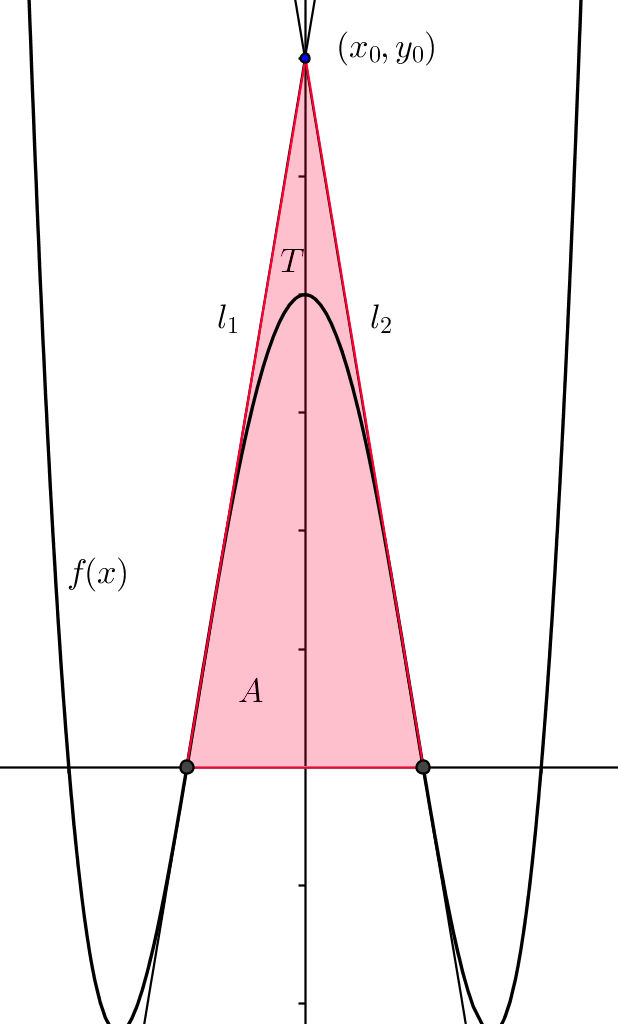
\includegraphics{tangential.PNG}}
\caption{Example figure for $f(x) = (1 - x^2) (2 - x) (2 + x)$ where $T$ is the area of the tangential triangle, $A$ is the area under $f$, $l_1$ and $l_2$ are the tangent lines at $x = \pm 1$.}
\end{figure}
\section*{Steps to Construct the Tangential Triangle}
To contruct the Tangential triangle we need to find the equation of the tangent line going through $x = \pm 1$ of $f$. We can do this by using some basic concepts from algebra. Using slope intercept form we get that:
\begin{align*}
\left\{ \begin{array}{lr} l_1 := y_1 = f'(-1)(x+1) \\ l_2 := y_2 = f'(1)(x-1).\end{array} \right.
\end{align*}
To find where they intersect we can simply set them equal to each other and we see that,
\begin{align*}
f'(-1)(x_0+1) = f'(1)(x_0-1) &\iff f'(-1)x_0 + f'(-1) = f'(1)x_0 - f'(1) \\&\iff f'(-1)x_0 - f'(1)x_0 = -f'(-1) - f'(1) \\&\iff x_0 = \frac{f'(-1)+ f'(1)}{f'(1) - f'(-1)} 
\end{align*}
And therefore,
\begin{align*}
y_0 = f'(1) \Big(\frac{f'(-1)+ f'(1)}{f'(1) - f'(-1)} - 1\Big) &\iff
y_0 = f'(1) \Big(\frac{f'(1) + f'(-1) - (f'(1) - f'(-1))}{f'(1)-f'(-1)}\Big) \\&\iff
y_0 = f'(1)\Big(\frac{2f'(-1)}{f'(1)-f'(-1)}\Big)
\end{align*}

\begin{proof}
We can rewrite $f(x) = (1-x^2) \prod_{i}(\alpha_i - x) \prod_{j}(\beta_j - x)$ since $f$ has real roots and $f(x) \neq 0$ for $x \in (-1, 1)$ for some $\alpha_{i}$ and $\beta_{j}$ that are both greater than or equal to 1.
\end{proof}
\end{document}